%http://math.mit.edu/~drew/
%https://math.stackexchange.com/questions/93689/software-for-galois-theory
%SetClassGroupBounds("GRH"); 
%K := QuadraticField(9);
%ClassNumber(K);

%https://en.wikipedia.org/wiki/List_of_triangle_inequalities

\documentclass[12pt, a4paper]{article}
\usepackage[bottom=2cm,top=3cm,left=3cm,right=2cm]{geometry}
\usepackage[utf8]{inputenc}
\usepackage{CJKutf8}
\usepackage{mathtext}
\usepackage{graphicx}
\usepackage{wrapfig}
\usepackage[T1]{fontenc}
\usepackage{blindtext}
\usepackage{tasks}
\usepackage{setspace}
\usepackage{amsmath}
\usepackage{amsfonts}
\usepackage{amssymb}
\usepackage{ wasysym }
\usepackage[portuguese]{babel}
\usepackage[utf8]{inputenc}
\usepackage{mathtext}
\usepackage{graphicx}
\usepackage{wrapfig}
\usepackage[T1]{fontenc}
\usepackage{blindtext}
\usepackage{setspace}
\usepackage{amsmath}
%\usepackage{geometry}
\usepackage{amsthm}
\usepackage{graphics}
%\usepackage{amsfonts}
%\usepackage{lipsum}
\usepackage{amssymb}
\usepackage{CJKutf8} %Pacote para escrever em japonês \begin{CJK}{UTF8}{min} \end{CJK}
\usepackage[portuguese]{babel}
\usepackage{multicol}
% \usepackage{colorspace}
\usepackage{graphicx, color}
\newcommand{\mdc}{{\rm mdc}}
\newcommand{\sen}{{\rm sen}}
\newcommand{\tg}{{\rm tg}}
\newcommand{\cotg}{{\rm cotg}}
\newcommand{\cossec}{{\rm cossec}}
\newcommand{\arctg}{{\rm arctg}}
\newcommand{\arcsen}{{\rm arcsen}}
\newcommand{\pulaquestao}{\newline\newline}
\newcommand{\negrito}[1]{\mbox{\boldmath{$#1$}}} 
\usepackage{pifont}
\newcommand{\heart}{\ensuremath\heartsuit}
\newcommand{\diamonde}{\ensuremath\diamondsuit}
\newtheorem{defi}{Definição}
\newtheorem{propo}{Proposição}
\newtheorem{dem}{Demonstração}
\newtheorem{coro}{Corolário}
\DeclareSymbolFont{extraup}{U}{zavm}{m}{n}
\DeclareMathSymbol{\varheart}{\mathalpha}{extraup}{86}
\DeclareMathSymbol{\vardiamond}{\mathalpha}{extraup}{87}
\setlength{\parindent}{0pt}
\usepackage[framemethod=TikZ]{mdframed}
%\usepackage{lipsum}
\mdfdefinestyle{MyFrame}{%
    linecolor=blue,
    outerlinewidth=2pt,
    roundcorner=20pt,
    innertopmargin=\baselineskip,
    innerbottommargin=\baselineskip,
    innerrightmargin=20pt,
    innerleftmargin=20pt,
    backgroundcolor=white!50!white}
    
%\mdfdefinestyle{Solução}{%
%    linecolor=blue,
%    outerlinewidth=1pt,
%    roundcorner=8pt,
%    innertopmargin=4pt%\baselineskip,
%    innerbottommargin=0pt%\baselineskip,
%    innerrightmargin=20pt,
%    innerleftmargin=20pt,
%    backgroundcolor=white!50!white}
    
    
    \mdfdefinestyle{DAS}{%
    linecolor=blue,
    outerlinewidth=2pt,
    roundcorner=20pt,
    innertopmargin=\baselineskip,
    innerbottommargin=\baselineskip,
    innerrightmargin=20pt,
    innerleftmargin=20pt,
    backgroundcolor=white!50!green}
% \definespotcolor{mygreen}{PANTONE 7716 C}{.83, 0, .00, .51}
% \definespotcolor{tuti}{}{0.6, 0, 1, .508}
\title{PIC - Programa de Iniciação Científica}
\author{Douglas de Araujo Smigly}
\date{30 de maio de 2020}
\begin{document}
\definecolor{Floresta}{rgb}{0.13,0.54,0.13}
\maketitle
\begin{center}
\large\textbf{\textcolor{Floresta}{Ciclo 2 - Encontro 2 - Probabilidade}}\\
\end{center}
%\begin{multicols*}{2}
%\setlength{\columnseprule}{0.78pt}
%\raggedcolumns
%\columnbreak
\textcolor{blue}{\bf(1)} (OBMEP 2016) A professora decidiu premiar, por sorteio, dois dentre os $20$ alunos da turma de João. Para o sorteio, $20$ bolas com os números dos alunos foram colocadas em uma caixa. A primeira bola sorteada pela professora caiu no chão e se perdeu, sem que ninguém visse seu número. Ela decidiu fazer o sorteio com as bolas restantes. Qual é a
probabilidade de que João tenha sido um dos dois alunos sorteados?
\newline\newline
\textcolor{blue}{\bf(2)} (OBMEP 2006) Uma caixa contém cinco bolas numeradas de 1 a 5. Dela são retiradas ao acaso duas
bolas. Qual a probabilidade de que o maior número assim escolhido seja o 4? \newline\newline
\textcolor{blue}{\bf(3)} (OBMEP 2015) Na figura, o círculo das centenas está dividido em três setores, um semicircular e
outros dois de mesma área. Cada um dos outros dois círculos está dividido em setores de mesma área. As setas nesses círculos, quando giradas, param ao acaso em algum setor, determinando um número de três algarismos. Por exemplo, na figura elas determinaram o número $331.$
\begin{figure}[!h]
    \centering
    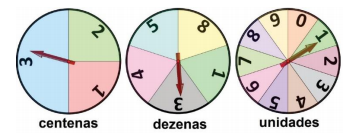
\includegraphics{Figuras/q3c2e2.png}
\end{figure}
Qual é a probabilidade de que o número determinado pelas setas, após serem giradas, seja maior do que $260?$
\newline\newline
\textcolor{blue}{\bf(4)} (OBMEP 2014) Dois dados têm suas faces pintadas de vermelho ou azul. Ao jogá-los, a probabilidade
de observarmos duas faces superiores de mesma cor é $\dfrac{11}{18}.$ Se um deles tem cinco faces vermelhas e uma azul, quantas faces vermelhas tem o outro?
\newline\newline
\textcolor{blue}{\bf(5)} (OBMEP 2013) Um dado foi construído usando a planificação da figura. Qual é a probabilidade de
obtermos dois resultados diferentes quando jogamos esse dado duas vezes?
\begin{figure}
    \centering
    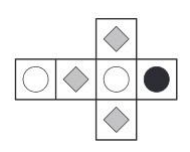
\includegraphics{Figuras/q5c2e2.png}
\end{figure}

\textcolor{blue}{\bf(6)} (OBMEP 2011) Três amigas possuem, cada uma, três blusas: uma amarela, uma branca e uma preta.
Se cada amiga escolher ao acaso uma de suas blusas, qual é a probabilidade de que as cores das blusas escolhidas sejam todas diferentes?
\newline\newline
\textcolor{blue}{\bf(7)} (OBMEP 2012) Pedro vai participar de um programa de prêmios em que há uma urna contendo
quatro bolas com valores diferentes e desconhecidos por ele, que serão sorteadas uma a uma até que ele decida ficar com uma delas. Ele observa o valor das duas primeiras bolas sorteadas e as descarta. Se o valor da terceira bola sorteada for maior que os das duas primeiras, ele ficará com ela e, caso contrário, ficará com a bola que restou. Qual é a probabilidade de Pedro ficar com a bola de maior valor?
\newline\newline
\textcolor{blue}{\bf(8)} Nove fichas, numeradas de $1$ a $9,$ são embaralhadas de modo aleatório, permanecendo uma sobre a outra. Se uma pessoa apostou que, na disposição final, as fichas estariam com as de número ímpar alternadas com as de número par. Qual é a probabilidade de ela ganhar?
\newline
\newline
\textcolor{blue}{\bf(9)} Colocam-se aleatoriamente $8$ bolas em $8$ urnas. Calcule a probabilidade de que exatamente uma urna seja deixada desocupada.
\newline
\newline
\textcolor{blue}{\bf(10)} Cinco homens e cinco mulheres sentam-se aleatoriamente em de cadeiras em círculo. Calcule a probabilidade de os homens e as mulheres se sentarem em lugares alternados.
\newline
\newline
\textcolor{blue}{\bf(11)} Em um armário há $10$ pares de sapatos distintos. Retiram-se, ao acaso, $4$ sapatos do armário. Qual é a probabilidade de se ter retirado pelo menos um par de sapatos?
\newline\newline
\textcolor{blue}{\bf(12) $\varheart$} Generalizando a questão anterior, suponha que no armário haja $n$ pares de sapatos. Retiram-se ao acaso $p$ pés de sapatos desse armário. Mostre que a probabilidade de haver entre esses pés exatamente $k$ pares de sapato é \[\dfrac{\dbinom{n}{k} \dbinom{n-k}{p-2k} 2^{p-2k}}{\dbinom{2n}{p}}.\]\newline \newline
\textcolor{blue}{\bf(13)} Doze pessoas são divididas em três grupos de 4. Qual é a probabilidade de duas determinadas pessoas ficarem no mesmo grupo?
\newline\newline
\textcolor{blue}{\bf(14) $\varheart$} Uma potência perfeita é um número inteiro da forma $a^b$, $a$ e $b$ inteiros, $b > 1$. Seja $f(n)$ a maior potência perfeita que não excede $n$ . Por exemplo, $f(7) = 4, f(8)=8$, e $f(99)=81$. Sorteando ao acaso um número inteiro $k$ com $1 \leq k \leq 100$ , qual a probabilidade de $f(k)$ ser um quadrado perfeito?
\begin{tasks}[counter-format={(tsk[a])},label-width=3.6ex, label-format = {\bfseries}, column-sep = {0pt}](5)
\task[\textcolor{Floresta}{$\negrito{(a)} $}] $64\%$
\task[\textcolor{Floresta}{$\negrito{(b)} $}] $72\%$
\task[\textcolor{Floresta}{$\negrito{(c)} $}] $81\%$
\task[\textcolor{Floresta}{$\negrito{(d)} $}] $90\%$
\task[\textcolor{Floresta}{$\negrito{(e)} $}] $96\%$
\end{tasks} 
%https://artofproblemsolving.com/community/c6h473647p2651848
\textcolor{blue}{\bf(15) $\varheart$} Um número $x$ é selecionado aleatoriamente do conjunto de números reais de modo que $5, 8$ e $x$ sejam lados de um triângulo. Qual é a probabilidade de que a área desse triângulo seja maior que $12$?%https://artofproblemsolving.com/community/q2h2163861p16060726\
\newline\newline
\textcolor{blue}{\bf(16) $\varheart$} Sejam $\alpha, \beta$ e $\gamma$ números aleatoriamente escolhidos, com reposição do conjunto $\{1,2,\ldots, 999\}.$ Qual é a probabilidade de que $\alpha^2 + \beta \gamma$ seja divisível por $3?$%https://artofproblemsolving.com/community/q1h2154662p15915689
\newline\newline
\textcolor{blue}{\bf(17) $\varheart$} Seja $0 < x < \dfrac{1}{6}$ um número real. Quando um certo dado viciado é rolado, uma face particular F ocorre com probabilidade $\dfrac{1}{6} - x$ e sua face oposta ocorre com probabilidade $\dfrac{1}{6} + x;$ as outras quatro faces ocorrem com probabilidade $\dfrac{1}{6}.$ Em qualquer dado, a soma de faces opostas é sempre $7.$ Assuma que a probabilidade de obter soma $7$ quando dois desses dados são rolados é $\dfrac{13}{96}.$ Qual é o valor de $x?$%https://artofproblemsolving.com/community/q1h1972212p13673835
\newline\newline
Exercícios marcados com $\varheart$ são extras.
\end{document}
SetClassGroupBounds("GRH"); 
K := QuadraticField(9);
ClassNumber(K);
Q := PolynomialRing(GF(2), 2);
Q;
K := QuadraticField();
G := GaloisGroup(K);
G;
\begin{CJK}{UTF8}{min}
露の世は 露の世ながら さりながら当時では老人と呼べる50歳代半ばでようやく授かったわが子への愛とその突然死を伝えた「露の世」のくだりは、その日記体句文集「おらが春」のクライマックスとなっています。

5月には数え二歳の誕生を迎えて詠んだ句に、
「這へ笑へ二つになるぞけさからは」と喜びを謳歌したばかり。

それが、翌6月にはもはや草葉の陰へと、その露の朝日に立ちどころに消えるごとく、儚くも身罷ってしまったとは。

人の世は朝露の如く無常なのだと、悔みを述べ慰問するあの人、この人。さは「さりながら」…それは確かにそうなのだけれども。
いかに「あきらめ顔しても、思い切りがたきは、恩愛のきづな也けり。」と、わが心中は耐えきれず切々と泣き崩れるばかり。わが子「さと」女を思う「大切」はやがて「あなた任せ」の境地へと通じていくものでしょう。
\end{CJK}